% Figure: CPG comparison across two environments (Acrobot vs Cartpole),
% same four arm configurations (random-shooting / CEM x MLP / TD-MPC2).
%
% Data sources:
%   Acrobot:
%     - RS x MLP-on-random-rollouts        : n=10, results/dmc_acrobot/cpg.json
%       CPG = +0.300, AC CI [-0.059, +0.559]
%     - RS x TD-MPC2 (2M)                  : n=10, results/dmc_acrobot/tdmpc2_cpg.json
%       CPG = +0.300, AC CI [-0.059, +0.559]
%     - CEM x MLP-on-TDMPC2-data, n=150    : results/dmc_acrobot/cem_cpg_sweep.json
%       CPG = +0.880, AC CI [+0.814, +0.923]
%     - CEM x TD-MPC2, n=150               : same JSON
%       CPG = +0.880, AC CI [+0.814, +0.923]
%   Cartpole (all four cells at n=30 pooled, model_size=5):
%     - RS x MLP-on-TDMPC2-data            : results/dmc_cartpole/coverage_mlp_on_tdmpc2_cpg_size5_pooled.json
%       CPG = +0.900, AC CI [+0.714, +0.973]
%     - RS x TD-MPC2 (1M, model_size=5)    : results/dmc_cartpole/tdmpc2_cpg_size5_pooled.json
%       CPG = +0.700, AC CI [+0.473, +0.840]
%     - CEM x MLP-on-TDMPC2-data           : results/dmc_cartpole/cem_cpg_size5_pooled.json
%       CPG = +0.500, AC CI [+0.285, +0.652]
%     - CEM x TD-MPC2                      : same JSON
%       CPG = +0.367, AC CI [+0.130, +0.558]
%
% AC error bars are asymmetric around the raw point estimate; we provide
% (eplus, eminus) per row.
%
% Note on sample-size asymmetry: the Acrobot random-shooting rows are at
% n=10 (not pooled to n=150) and inherit the wider CI of the v0.10/v0.11
% headline; the Acrobot CEM rows are pooled-150; all Cartpole rows are
% pooled-n=30. We label this in the caption rather than overlay sample-size
% glyphs in the figure.
\begin{figure}[t]
  \centering
  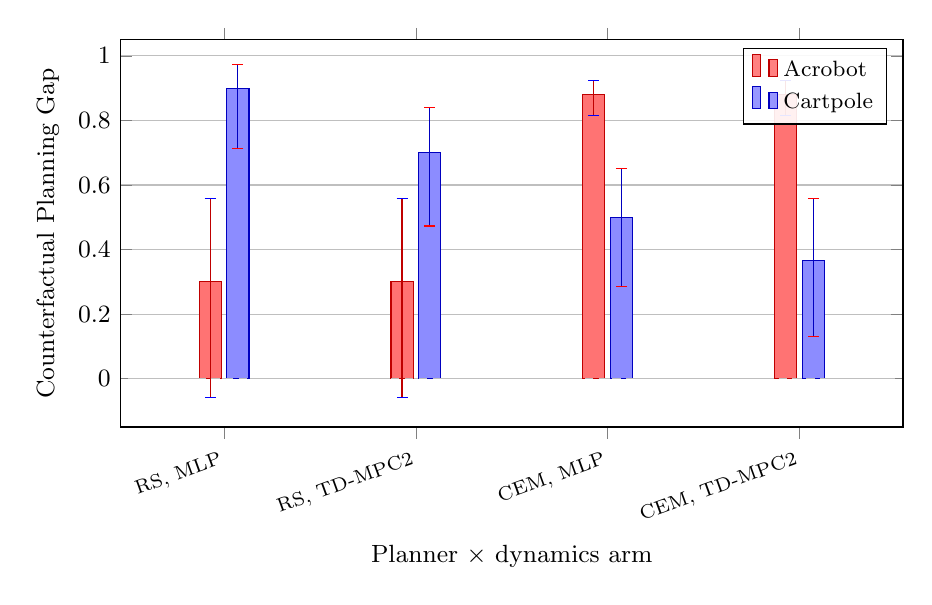
\begin{tikzpicture}
    \begin{axis}[
        width=0.95\columnwidth,
        height=6.5cm,
        font=\small,
        ybar=2pt,
        bar width=8pt,
        ymin=-0.15, ymax=1.05,
        ytick={0, 0.2, 0.4, 0.6, 0.8, 1.0},
        ylabel={Counterfactual Planning Gap},
        ymajorgrids=true,
        xtick={1, 2, 3, 4},
        xticklabels={
          {RS, MLP},
          {RS, TD-MPC2},
          {CEM, MLP},
          {CEM, TD-MPC2},
        },
        x tick label style={font=\scriptsize, rotate=20, anchor=north east},
        xlabel={Planner $\times$ dynamics arm},
        legend cell align=left,
        legend style={
          at={(0.98, 0.98)}, anchor=north east,
          font=\footnotesize,
          fill=white, fill opacity=0.9, draw opacity=1, text opacity=1,
        },
        enlarge x limits=0.18,
      ]
      \addplot+[
          fill=red!55, draw=red!75!black,
          error bars/.cd, y dir=both, y explicit,
        ]
        table[x=x, y=y, y error plus=eplus, y error minus=eminus, row sep=\\] {
          x y     eplus eminus \\
          1 0.300 0.259 0.359  \\
          2 0.300 0.259 0.359  \\
          3 0.880 0.043 0.066  \\
          4 0.880 0.043 0.066  \\
        };
      \addlegendentry{Acrobot}
      \addplot+[
          fill=blue!45, draw=blue!75!black,
          error bars/.cd, y dir=both, y explicit,
        ]
        table[x=x, y=y, y error plus=eplus, y error minus=eminus, row sep=\\] {
          x y     eplus eminus \\
          1 0.900 0.073 0.186  \\
          2 0.700 0.140 0.227  \\
          3 0.500 0.152 0.215  \\
          4 0.367 0.191 0.237  \\
        };
      \addlegendentry{Cartpole}
      \draw[densely dashed, gray!50] (axis cs:0.5, 0) -- (axis cs:4.5, 0);
    \end{axis}
  \end{tikzpicture}
  \caption{Cross-environment CPG with Agresti--Caffo $95\%$ CI error bars. Same four planner-dynamics combinations on two envs. Sample sizes: Acrobot random-shooting cells at $n = 10$, Acrobot CEM cells pooled at $n = 150$, Cartpole all four cells pooled at $n = 30$ (TD-MPC2 \texttt{model\_size}~$= 5$). The \textsc{model bottleneck} verdict reproduces in every cell; the gap magnitude differs and ranks the four arm configurations consistently within each env. The TD-MPC2 arm on Cartpole reaches non-zero learned-arm success ($0.200$ random-shooting, $0.133$ CEM), so the gap shrinks but stays bounded above zero -- the metric tracks gap magnitude, not just gap presence.}
  \label{fig:cross_env_cpg}
\end{figure}
